\documentclass[11pt,a4paper]{article}
\usepackage[margin=22mm]{geometry}
\usepackage[T1]{fontenc}
\usepackage{tikz}
\usepackage{booktabs}
\usepackage{longtable}
\usepackage{array}
\usepackage{hyperref}
\usetikzlibrary{arrows.meta, positioning, shapes.geometric}
\newcolumntype{L}[1]{>{\raggedright\arraybackslash}p{#1}}
\title{Canonical CBOR snapshots carried by \texttt{ir\_stream} --- implementation plan}
\author{Claude (core\_cpp agent), working in hymeko/core}
\date{Created-at: 2026-09-15 21:13 CEST}

\begin{document}
\sloppy
\maketitle

\section*{Authorisation}

\begin{quote}
\texttt{APPROVED-CORE-EDIT: ir-stream-cbor-snapshot}
\end{quote}

The user supplied this token verbatim in the core\_cpp Claude Code chat on 2026-09-15 (turn after 21:07 CEST),
after two decisions in the same chat: the Core extension is wanted (``Core-bővítés is''), the Rust Core change goes on
its own branch (``a rust core IR külön branchen menjen''), and the complete IR snapshot stays canonical CBOR
(``CBOR nem messagepack''). The token covers exactly the boundary in Section~3; the commit message, if the user later
authorises one, repeats it in a footer. No commit or push is authorised by this plan.

Git state recorded before the plan: \texttt{git fetch origin} succeeded at 21:03 CEST;
\texttt{origin/main} = \texttt{368c7fda59cc1ae4834d41581841778e57d677ba}. The existing checkout
\texttt{hymeko\_framework/core} is on \texttt{perf/compiler-repeated-work} with another worker's uncommitted
\texttt{ir-value-updates} edits (\texttt{execution.rs}, \texttt{execution/value\_updates.rs}); it is not switched or
touched. \textbf{Worktree exception}: reason --- the only checkout carries another worker's dirty branch; path
\texttt{D:/hakiko\_ai\_ws/03\_implementation/worktrees/core-ir-stream-cbor-snapshot}; branch
\texttt{feat/ir-stream-cbor-snapshot} from \texttt{origin/main} (upstream unset so no push can target main); owner ---
this core\_cpp agent; retirement --- after merge or abandonment, inspect for dirty files and unpublished commits
before removal.

\section*{ETA}

About 2.5 hours, completion near 2026-09-15 23:45 CEST. Basis: plan and PDF 30 min; section kind and CBOR stream
bridge with unit tests 50 min; integration test 20 min; first cold build of \texttt{hymeko\_core} in the new worktree
plus targeted tests 25 min (\texttt{-j 8}); fmt, clippy, symbols, duplication 15 min; report and archive 15 min.

\section{Goal and ownership}

A complete, validated HyMeKo IR must travel over the existing \texttt{ir\_stream} transaction protocol
(\texttt{SnapshotBegin} $\to$ \texttt{SnapshotChunk}$^{*}$ $\to$ \texttt{Commit}) in fragments small enough for a
UART link and large enough for a LAN, and a consumer must turn a committed transaction into a Core-validated IR
without source parsing. Two consumers need this now: the robotics HIVE store over Zenoh (another agent,
\texttt{robotics/docs/plans/2026-09-12-belief-planner/plan.md}, ``LAN HIVE implementation'') and, later, the
core\_cpp MCU runtime over the ST-LINK virtual COM port.

Ownership, verified against code: \texttt{hymeko\_core::ir\_stream} owns the wire vocabulary, validation and
transaction admission; its assembler explicitly does not apply transactions. \texttt{writers::cbor\_writer} is ``the
only owner of the CBOR schema'' and already depends on \texttt{ir\_stream::DecodeLimits}. Today no section kind can
carry declarations, hierarchy, symbols or imports (\texttt{section.rs} defines ten numeric kinds;
\texttt{ElementKind::Raw8} exists for opaque bodies). This plan therefore adds one opaque section kind to
\texttt{ir\_stream} and the CBOR-specific producer and consumer to the CBOR owner. It adds no second codec, no
dependency and no IR schema.

\section{Discovery ledger}

\begin{small}
\begin{verbatim}
DISCOVERY LEDGER - canonical-CBOR snapshot carriage over ir_stream
  find:    find hymeko_core/src/{writers,ir_stream} hymeko_core/tests
           -iname "*snapshot*" -o -iname "*stream*"
           -> 2 hits: src/ir_stream (dir), tests/ir_stream_admission.rs
  grep:    grep -rnE "CanonicalIr|cbor[_ ]snapshot|snapshot[_ ]cbor|IrCbor"
           hymeko_core/src hymeko_core/tests docs -> 0 hits
           grep -rlE SnapshotChunk hymeko_core/{src,tests,benches} -> 4 hits:
           src/ir_stream/{assembler,codec,envelope}.rs, benches/ir_stream_bench.rs
           (vocabulary and tests; no CBOR producer)
           axon, hive, robotics *.rs: SnapshotBegin|encode_message|CanonicalIr|
           ir_stream -> 0 hits; "SectionKind::" outside core -> 0 hits
  symbols: SYMBOLS.md -> CborPayload, DecodedCborPayload, CborError;
           CommittedTransaction, StagedSection, TransactionAssembler,
           EnvelopeDraft, MessageType, SectionEntry, ElementKind, DecodeLimits
  read:    ir_stream/{mod,section,codec,limits,assembler,envelope,version}.rs,
           writers/cbor_writer.rs, cbor_writer/tests.rs, tests/mod.rs,
           tests/ir_stream_admission.rs, tests/unified_ir/validation/
           cbor_roundtrip.rs, docs/hypergraph-synchronization.md 4-6,
           docs/plans/2026-09-04-canonical-cbor-codec, robotics LAN HIVE plan
  verdict: EXTEND src/ir_stream/section.rs + NEW
           src/writers/cbor_writer/stream.rs; rejected the bridge inside
           ir_stream (transport vocabulary must not depend on the CBOR owner)
           and a MessagePack writers/snapshot.rs (user: CBOR, not MessagePack)

DISCOVERY LEDGER - tests/ir_stream_cbor_snapshot.rs
  verdict: NEW, wired through tests/mod.rs; rejected ir_stream_admission.rs
           (charter: admission with empty tables, not installation) and
           cbor_roundtrip.rs (CBOR facade only; carries memory probes)

DISCOVERY LEDGER - docs/plans/2026-09-15-ir-stream-cbor-snapshot
  find:    ls docs/plans | grep -iE "stream|cbor|snapshot" -> 2 hits:
           2026-08-28-ir-stream-wire-codec, 2026-09-04-canonical-cbor-codec
  verdict: NEW; both hits are completed phases under other approval slugs
\end{verbatim}
\end{small}

\section{Approved boundary (CORE.YAML items touched)}

\begin{longtable}{@{}L{0.43\linewidth}L{0.33\linewidth}L{0.16\linewidth}@{}}
\toprule
Path & Change & Authority \\
\midrule
\texttt{hymeko\_core/src/ir\_stream/section.rs} & variant \texttt{SectionKind::CanonicalIrCbor} = wire 11, mapping,
rustdoc, unit tests & approved core \\
\texttt{hymeko\_core/src/writers/cbor\_writer.rs} & \texttt{mod stream;} and re-exports & approved core \\
\texttt{hymeko\_core/src/writers/cbor\_writer/stream.rs} (new) & producer, consumer, error type & approved core \\
\texttt{hymeko\_core/src/writers/cbor\_writer/tests.rs} & unit tests reusing the existing fixture & approved core \\
\texttt{CORE.YAML} & \texttt{approved\_edits} record of this slug & approved core \\
\texttt{hymeko\_core/tests/ir\_stream\_cbor\_snapshot.rs} (new), \texttt{tests/mod.rs} & integration test &
allowlisted \\
\texttt{docs/hypergraph-synchronization.md} \S5.3 & table row; implemented versus specified kinds & not core \\
\texttt{SYMBOLS.md} & regenerated & generated \\
\texttt{docs/plans/**}, \texttt{reports/**} & traceability & allowlisted \\
\bottomrule
\end{longtable}

Out of scope: MessagePack or any new codec; dependency or \texttt{Cargo.toml}/\texttt{Cargo.lock} changes; IR schema,
canonical hash, CBOR wire bytes; the envelope, section validator and assembler logic (only the kind mapping grows);
installation into \texttt{ExecutionState}/\texttt{CompiledModel} (\texttt{execution.rs}, the HIVE agent's
\texttt{ir-value-updates} area); delta semantics for IR structure; authenticity (the codec documents it as a transport
concern); the C consumer in core\_cpp; commit, push, merge.

\section{Interface changes}

\begin{small}
\begin{verbatim}
// hymeko::ir_stream::section
pub enum SectionKind { ..., CanonicalIrCbor, Unknown(u16) }  // wire 11, critical,
                                                             // repeatable, not skippable
// hymeko::writers::cbor_writer (re-exported from the child module `stream`)
pub struct SnapshotMessageDraft {
    pub stream_id: u64, pub first_seq: u64, pub txn_id: u64,
    pub base_version: SnapshotVersion, pub target_version: SnapshotVersion,
    pub max_fragment_bytes: usize,
}
pub fn encode_snapshot_messages(cbor: &[u8], draft: &SnapshotMessageDraft)
    -> Result<Vec<Vec<u8>>, CborStreamError>;
pub fn decode_snapshot(transaction: &CommittedTransaction, limits: &DecodeLimits)
    -> Result<DecodedCborPayload, CborStreamError>;
pub enum CborStreamError {
    EmptyDocument, ZeroFragmentSize, SequenceOverflow,
    NotASnapshot { kind: TransactionKind },
    NoFragments,
    UnexpectedSection { index: usize, kind: SectionKind },
    WrongElementKind { index: usize, got: ElementKind },
    TooLarge { got: u64, max: u64 },
    Cbor(CborError),
}
\end{verbatim}
\end{small}

\section{Contracts}

\paragraph{Wire.} \texttt{CanonicalIrCbor} sections carry \texttt{ElementKind::Raw8} bodies whose concatenation, in
staging order (message order, then table order), is one canonical CBOR document of
\texttt{hymeko/model/ir/cbor/v1}. The kind is below \texttt{CRITICAL\_SECTION\_MAX}, so an older consumer refuses it
with \texttt{UnknownMandatorySection} instead of skipping meaning. It is repeatable, so one document may span any
number of chunks; existing numeric kinds keep their singleton and patch rules unchanged.

\paragraph{Producer.} Preconditions: \texttt{cbor} is non-empty and was produced by \texttt{encode} or
\texttt{encode\_compiled}; \texttt{max\_fragment\_bytes} $> 0$; \texttt{first\_seq} is the stream's next sequence
number; \texttt{target\_version} obeys the assembler's rules (a topology bump also bumps weights and features).
Postcondition: messages \texttt{SnapshotBegin} (empty section table), one \texttt{SnapshotChunk} per fragment with a
single \texttt{CanonicalIrCbor} section and \texttt{FLAG\_LAST\_CHUNK} on the last, then \texttt{Commit}; contiguous
sequence numbers checked for overflow; every message passes \texttt{validate\_message} under limits that admit one
fragment (\texttt{max\_section\_bytes} $\ge$ fragment, \texttt{max\_payload\_bytes} $\ge 40 +$ fragment). The producer
does not decode the document; the consumer is the validation authority.

\paragraph{Consumer.} Preconditions: \texttt{transaction} came from \texttt{TransactionAssembler::apply}; the caller's
\texttt{AssemblerLimits} admit the document (\texttt{max\_staged\_bytes}, \texttt{max\_staged\_sections},
\texttt{max\_chunks}). Rules, in order: the kind is \texttt{Snapshot}; at least one section; every section is
\texttt{CanonicalIrCbor} (a CBOR snapshot is the complete state, so a numeric section beside it would be a second
authority) with \texttt{Raw8} elements; the checked total length is at most \texttt{limits.max\_message\_bytes},
tested before the concatenation buffer is allocated; then \texttt{cbor\_writer::decode} with the same limits.
Postcondition: the returned \texttt{DecodedCborPayload} satisfies every existing CBOR boundary check (preflight,
schema, IDs, index, coherence, recomputed canonical hash). Failure leaves nothing published; this function holds no
state.

\paragraph{Invariants.} Envelope validation, section-table validation, digest coverage, replay and version admission
are unchanged. \texttt{decode(encode(x))} identity carries over: a document sent in any fragmentation decodes to the
same canonical hash as a direct \texttt{decode}.

\section{Test strategy (correctness only)}

\begin{enumerate}
\item \textbf{Unit, \texttt{section.rs}}: wire 11 round-trips; the kind is neither singleton nor skippable; a table
with two \texttt{CanonicalIrCbor} sections validates; values 12--999 still reject as unknown mandatory.
\item \textbf{Unit, \texttt{cbor\_writer/tests.rs}} (existing one-node fixture, real \texttt{validate\_message} and
\texttt{TransactionAssembler}): fragment sizes 1, 3, exact length and larger than the document round-trip to the
direct-decode canonical hash; message count, flags, contiguous sequence and per-message validation. Negative controls:
empty document, zero fragment size, sequence overflow, a \texttt{Delta} transaction, a snapshot without sections, a
mixed numeric section, a non-\texttt{Raw8} section, a total above \texttt{max\_message\_bytes}, a dropped middle
fragment and two swapped fragments (both must fail \texttt{decode}).
\item \textbf{Integration, \texttt{tests/ir\_stream\_cbor\_snapshot.rs}}: every lowerable corpus fixture
(\texttt{require\_fixtures}, fail-closed) is encoded with \texttt{encode\_compiled}, split into 4096-byte fragments,
driven through the public wire validator and assembler, and decoded; canonical hash, root path, imports and declaration
count equal the direct decode. One fixture repeats with fragment sizes 1 and 257.
\item \textbf{Regression}: \texttt{cargo test -p hymeko\_core --lib ir\_stream}, \texttt{--lib writers::cbor\_writer},
\texttt{--test mod ir\_stream\_admission}, and the functional \texttt{cbor\_roundtrip} tests selected by exact name
after inspection. The \texttt{canonical\_cbor\_memory\_*} evidence probes and every benchmark stay unrun.
\item \textbf{Static gates}: \texttt{cargo fmt --all -- --check}; \texttt{cargo clippy -p hymeko\_core --all-targets --
-D warnings}; \texttt{contract-symbols --root . --check} after regeneration; \texttt{contract-duplication --root .}
against the baseline.
\end{enumerate}

Every test selection is inspected first: the aggregate \texttt{mod} test crate also contains opt-in profile modules,
so only filtered test names run.

\section{Performance budget}

No benchmark, profile or timing measurement is authorised or run. Resource bounds are structural: the consumer
allocates one buffer of the checked document length (at most \texttt{DecodeLimits::max\_message\_bytes}, default
256~MiB) in addition to the assembler's staged fragments, so peak memory is about twice the document plus the decoded
IR. The producer allocates one \texttt{Vec<u8>} per message ($144 + 40 +$ fragment bytes). Build jobs are limited to 8
to stay far below the 16~GB RSS cap, which Windows cannot enforce with \texttt{systemd-run}.

\section{Rollback}

All changes stay uncommitted on \texttt{feat/ir-stream-cbor-snapshot}. Rollback is \texttt{git restore} and deletion of
the new files in the worktree, or removal of the branch and worktree after inspection. Wire value 11 is unpublished
until a merge, so no persisted message or fixture depends on it.

\section{Risk anticipation}

\begin{itemize}
\item \textbf{Performance-contract preservation.} The section validator, envelope, digest, assembler limits and
replay window keep every existing check; the only validator change is one more accepted kind below the critical
boundary. Staging limits still bound the fragment count and staged bytes; the consumer adds a length check before its
single allocation, so the new path inherits the ``limits before allocation'' contract.
\item \textbf{Worst-case input.} A hostile or buggy stream sends many 1-byte fragments (bounded by
\texttt{max\_chunks}/\texttt{max\_staged\_sections}), fragments whose sum exceeds the limit (rejected before
allocation), reordered or missing fragments (rejected by CBOR preflight, validation or canonical hash), or valid CBOR
of a different model (accepted as that model: authenticity is a transport concern and stays documented as such).
Production documents are robot and planner models from kilobytes to megabytes; the default limits leave headroom.
\item \textbf{Wire-number collision.} Another unpublished branch could claim kind 11. Remote branches show no
\texttt{ir\_stream} work; the concurrent \texttt{ir-value-updates} edits touch \texttt{execution.rs} only.
\item \textbf{Exhaustive matches.} Adding a public enum variant breaks exhaustive matches in dependants. No crate
outside core in the workspace matches on \texttt{SectionKind}.
\item \textbf{Version rule surprise.} Producers that bump topology alone are rejected by the assembler; the producer
rustdoc states the rule and a test drives it.
\item \textbf{Memory of large snapshots.} Concatenation doubles the document transiently; a streaming decoder is not
possible without changing the CBOR preflight, which is out of scope.
\item \textbf{Scope creep into the HIVE agent's area.} No edit to \texttt{module\_store}; the hand-off point is the
validated \texttt{DecodedCborPayload}.
\end{itemize}

\section{Tooling notes}

\texttt{mmdc} is absent on this host (\texttt{tools.yaml}); \texttt{plan.mmd} is source only. Clippy runs for
\texttt{hymeko\_core} with all targets instead of the whole workspace, because \texttt{hymeko\_wgpu} is untouched.
The contract gates run through the installed entry points pinned by \texttt{tools/hooks} (provider
\texttt{8871abe}).

\section*{Architecture}
\begin{center}
\resizebox{\linewidth}{!}{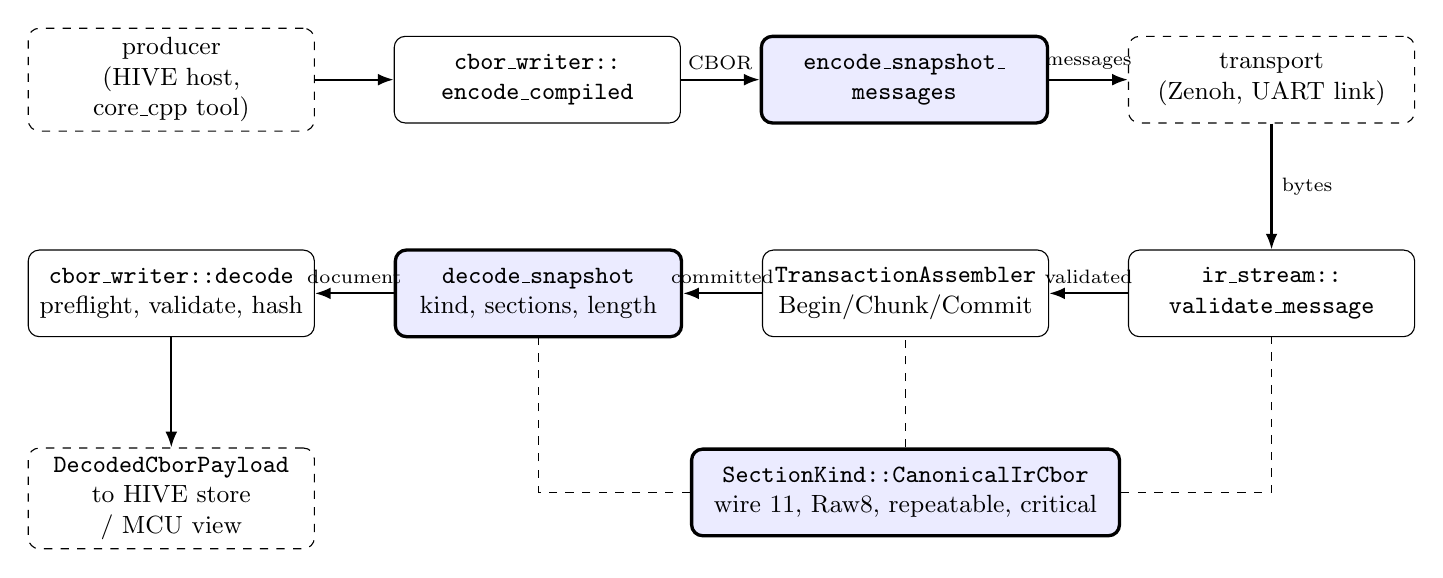
\begin{tikzpicture}[
  box/.style={draw, rounded corners, align=center, minimum height=11mm, text width=34mm, font=\small},
  new/.style={box, very thick, fill=blue!8},
  ext/.style={box, dashed},
  arr/.style={-{Latex[length=2mm]}, thick},
  lbl/.style={font=\scriptsize, align=center}
]
\node[ext] (prod) {producer\\(HIVE host, core\_cpp tool)};
\node[box, right=10mm of prod] (enc) {\texttt{cbor\_writer::}\\\texttt{encode\_compiled}};
\node[new, right=10mm of enc] (msgs) {\texttt{encode\_snapshot\_}\\\texttt{messages}};
\node[ext, right=10mm of msgs] (wire) {transport\\(Zenoh, UART link)};

\node[box, below=16mm of wire] (val) {\texttt{ir\_stream::}\\\texttt{validate\_message}};
\node[box, left=10mm of val] (asm) {\texttt{TransactionAssembler}\\Begin/Chunk/Commit};
\node[new, left=10mm of asm] (dec) {\texttt{decode\_snapshot}\\kind, sections, length};
\node[box, left=10mm of dec] (cbor) {\texttt{cbor\_writer::decode}\\preflight, validate, hash};

\node[ext, below=14mm of cbor] (cons) {\texttt{DecodedCborPayload}\\to HIVE store / MCU view};
\node[new, below=14mm of asm, text width=52mm] (kind) {\texttt{SectionKind::CanonicalIrCbor}\\wire 11, Raw8, repeatable, critical};

\draw[arr] (prod) -- (enc);
\draw[arr] (enc) -- node[lbl, above]{CBOR} (msgs);
\draw[arr] (msgs) -- node[lbl, above]{messages} (wire);
\draw[arr] (wire) -- node[lbl, right]{bytes} (val);
\draw[arr] (val) -- node[lbl, above]{validated} (asm);
\draw[arr] (asm) -- node[lbl, above]{committed} (dec);
\draw[arr] (dec) -- node[lbl, above]{document} (cbor);
\draw[arr] (cbor) -- (cons);
\draw[dashed] (kind) -- (asm);
\draw[dashed] (kind.west) -| (dec.south);
\draw[dashed] (kind.east) -| (val.south);
\end{tikzpicture}
}
\end{center}

\end{document}
